% !TEX TS-program = pdflatexmk
% mnras_template.tex
%
% LaTeX template for creating an MNRAS paper
%
% v3.0 released 14 May 2015
% (version numbers match those of mnras.cls)
%
% Copyright (C) Royal Astronomical Society 2015
% Authors:
% Keith T. Smith (Royal Astronomical Society)

% Change log
%
% v3.0 May 2015
%    Renamed to match the new package name
%    Version number matches mnras.cls
%    A few minor tweaks to wording
% v1.0 September 2013
%    Beta testing only - never publicly released
%    First version: a simple (ish) template for creating an MNRAS paper

%%%%%%%%%%%%%%%%%%%%%%%%%%%%%%%%%%%%%%%%%%%%%%%%%%

\documentclass[a4paper,fleqn,usenatbib]{mnras}

\usepackage{newtxtext,newtxmath}
\usepackage[T1]{fontenc}
\usepackage{ae,aecompl}
\usepackage{graphicx}	% Including figure files
\usepackage{amsmath}	% Advanced maths commands
\usepackage{amssymb}	% Extra maths symbols

%%%%%%%%%%%%%%%%%%%%%%%%%%%%%%%%%%%%%%%%%%%%%%%%%%

\title[Gaussian Process Spectra]{Gaussian Process Spectra}
\author[S. M. Feeney et al.]{
Stephen M. Feeney,$^{1}$\thanks{E-mail: sfeeney@flatironinstitute.org}
Benjamin D. Wandelt,$^{1,2,3,4}$
and Melissa K. Ness$^{1,5}$
\\
$^{1}$Center for Computational Astrophysics, Flatiron Institute, 162 Fifth Avenue, New York, NY 10010, USA\\
$^{2}$Institut d'Astrophysique de Paris (IAP), UMR 7095, CNRS UPMC Universit\'e Paris 6, Sorbonne Universit\'es, \\
98bis boulevard Arago, F-75014 Paris, France\\
$^{3}$Institut Lagrange de Paris (ILP), UMR 7095, CNRS UPMC Universit\'e Paris 6, Sorbonne Universit\'es, \\
98bis boulevard Arago, F-75014 Paris, France\\
$^{4}$Department of Physics and Astronomy, University of Illinois at Urbana-Champaign, 1002 W Green St, Urbana, IL 61801, USA\\
$^{5}$Department of Astronomy, Columbia University, Pupin Physics Laboratories, New York, NY 10027, USA
}

% These dates will be filled out by the publisher
\date{Accepted XXX. Received YYY; in original form ZZZ}

% Enter the current year, for the copyright statements etc.
\pubyear{2019}

% Don't change these lines
\begin{document}
\label{firstpage}
\pagerange{\pageref{firstpage}--\pageref{lastpage}}
\maketitle

% Abstract of the paper
\begin{abstract}
This is a simple template for authors to write new MNRAS papers.
The abstract should briefly describe the aims, methods, and main results of the paper.
It should be a single paragraph not more than 250 words (200 words for Letters).
No references should appear in the abstract.
\end{abstract}

% Select between one and six entries from the list of approved keywords.
% Don't make up new ones.
\begin{keywords}
keyword1 -- keyword2 -- keyword3
\end{keywords}

%%%%%%%%%%%%%%%%%%%%%%%%%%%%%%%%%%%%%%%%%%%%%%%%%%

\section{Introduction}

Stuff.

%%%%%%%%%%%%%%%%%%%%%%%%%%%%%%%%%%%%%%%%%%%%%%%%%%

\section{Methods}

More stuff.

\begin{figure}
	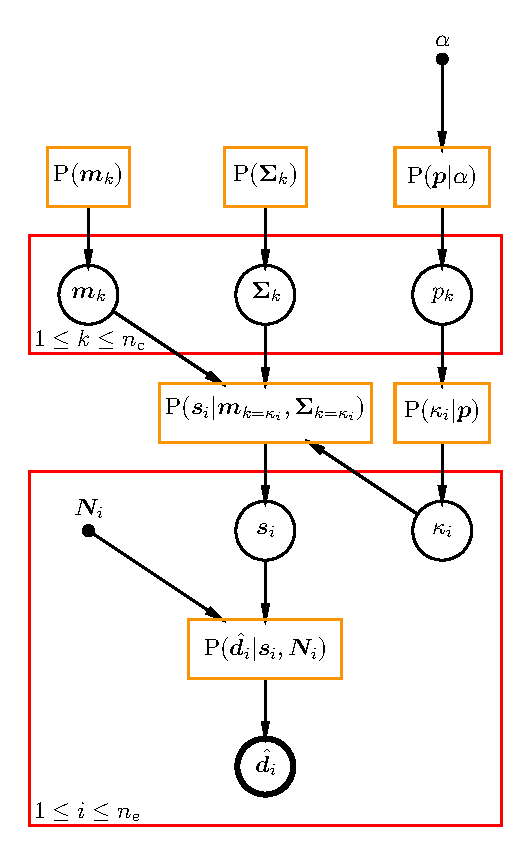
\includegraphics[width=\columnwidth]{bhm_plot.pdf}
    \caption{Network diagram for our hierarchical Bayesian model.}
    \label{fig:network_diagram}
\end{figure}

%%%%%%%%%%%%%%%%%%%%%%%%%%%%%%%%%%%%%%%%%%%%%%%%%%

\section{Results}

Even more stuff.

\begin{figure*}
	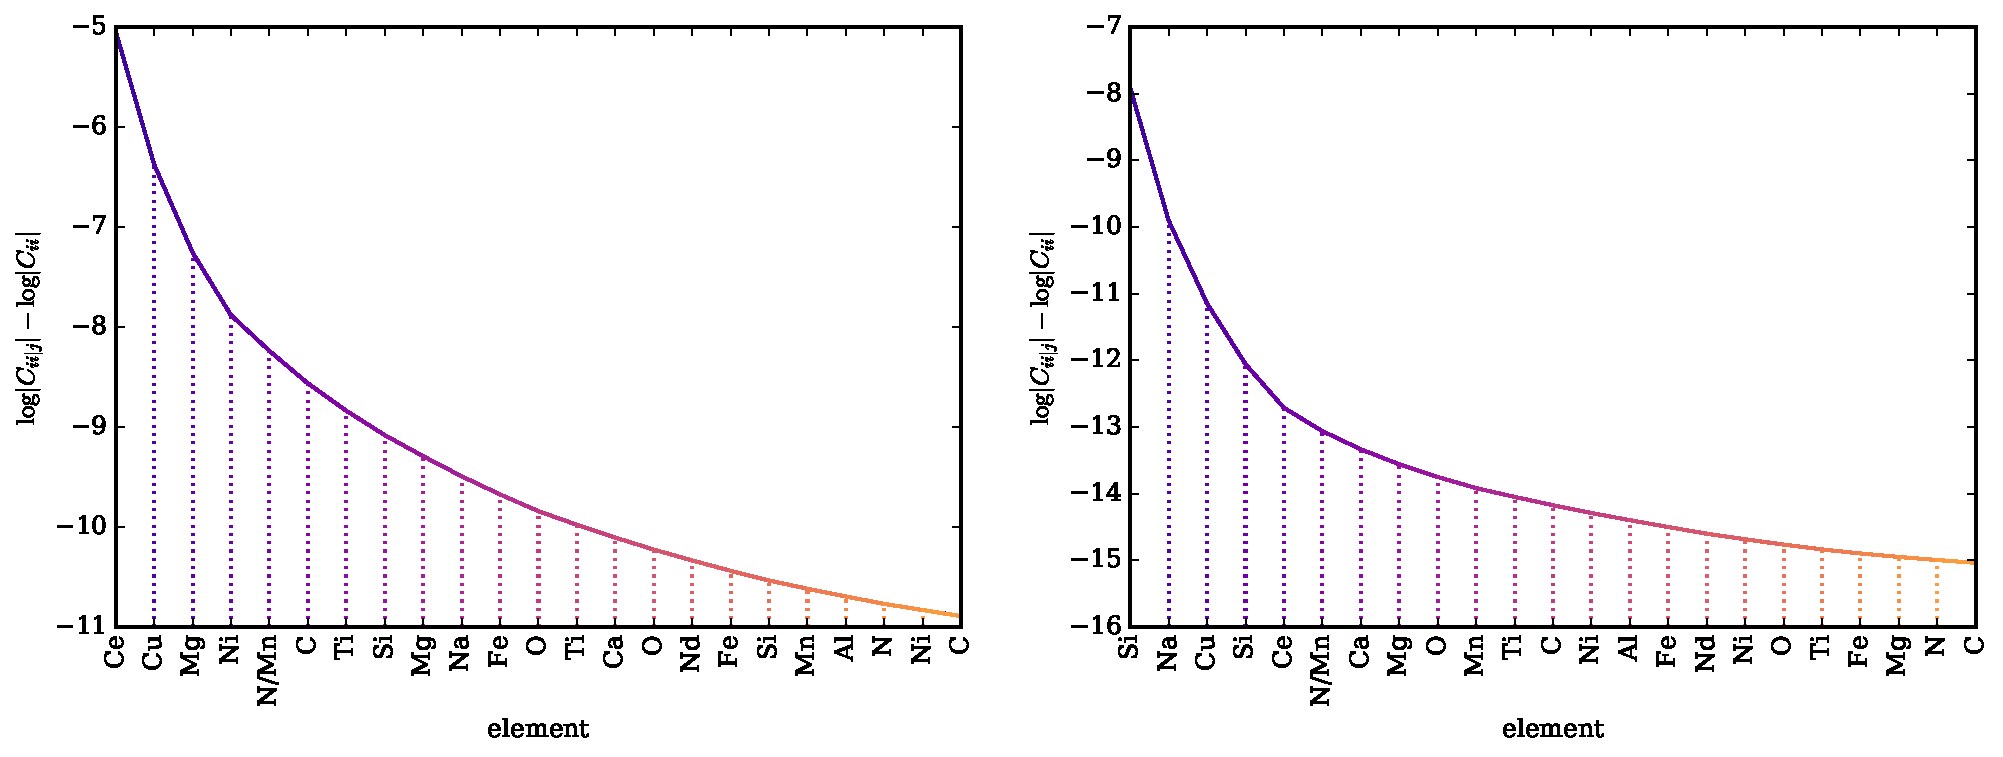
\includegraphics[width=2\columnwidth]{apogee_centers_subset2_ce_nd_29502_spc_ce_inf_gain.pdf}
	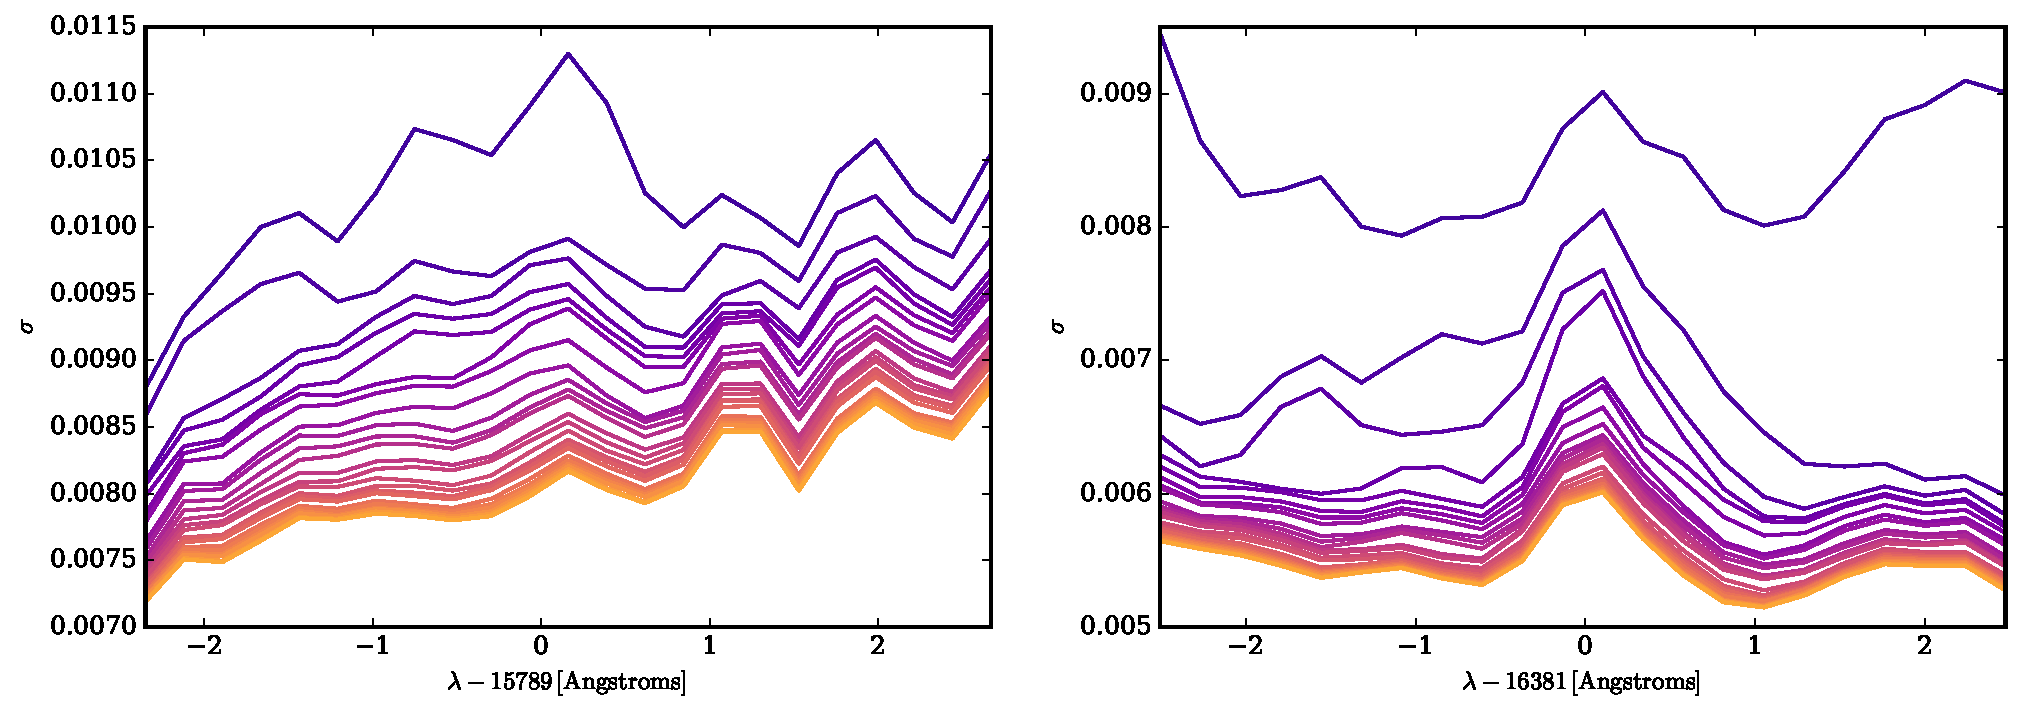
\includegraphics[width=2\columnwidth]{apogee_centers_subset2_ce_nd_29502_spc_ce_conditional_stddevs.pdf}
    \caption{Information gain (top) and conditional standard deviation (bottom) for Cerium windows given observations of other elemental windows.}
    \label{fig:ce_information}
\end{figure*}

\begin{figure}
	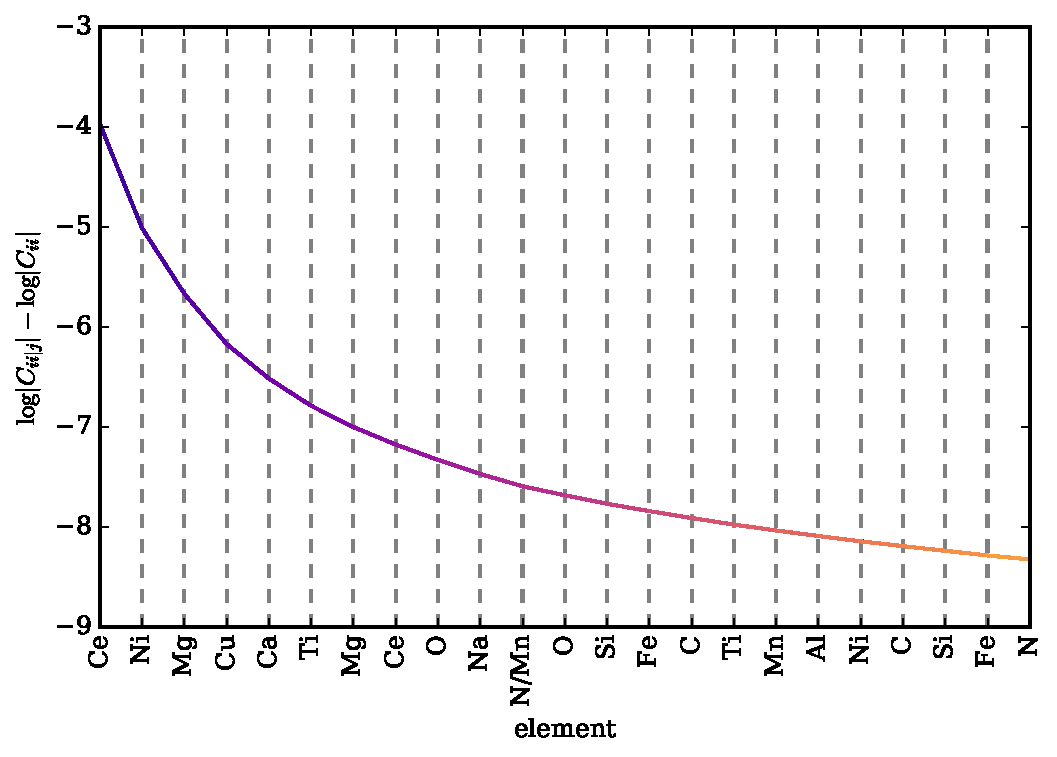
\includegraphics[width=\columnwidth]{apogee_centers_subset2_ce_nd_29502_spc_nd_inf_gain.pdf}
	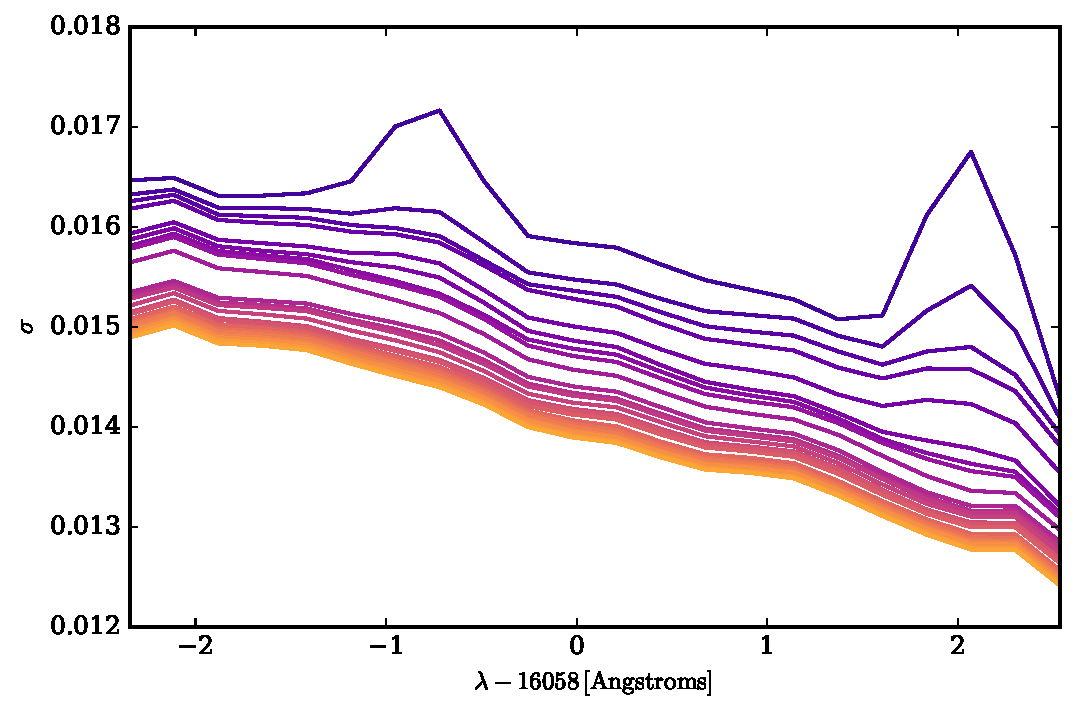
\includegraphics[width=\columnwidth]{apogee_centers_subset2_ce_nd_29502_spc_nd_conditional_stddevs.pdf}
    \caption{Information gain (top) and conditional standard deviation (bottom) for Neodymium window given observations of other elemental windows.}
    \label{fig:nd_information}
\end{figure}

%%%%%%%%%%%%%%%%%%%%%%%%%%%%%%%%%%%%%%%%%%%%%%%%%%

\section{Conclusions}

TBD.

%%%%%%%%%%%%%%%%%%%%%%%%%%%%%%%%%%%%%%%%%%%%%%%%%%

\section*{Acknowledgements}

The Flatiron Institute is supported by the Simons Foundation.

%%%%%%%%%%%%%%%%%%%%%%%%%%%%%%%%%%%%%%%%%%%%%%%%%%

%\bibliographystyle{mnras}
%\bibliography{example} % if your bibtex file is called example.bib

%%%%%%%%%%%%%%%%%%%%%%%%%%%%%%%%%%%%%%%%%%%%%%%%%%


% Don't change these lines
\bsp	% typesetting comment
\label{lastpage}
\end{document}

% End of mnras_template.tex